Labeling the expensive MC TBR model $f(x)$, a surrogate is a mapping
$\hat{f}(x)$ such that $f(x)$ and $\hat{f}(x)$ minimise a selected dissimilarity
metric. In order to be considered \textit{viable}, $\hat{f}(x)$ is required to
achieve expected evaluation time lower than that of~$f(x)$. In this work, we
consider two methods of producing viable surrogates: (1) a conventional decoupled
approach, which evaluates $f(x)$ on a set of randomly sampled points and
trains surrogates in a supervised scheme, and (2) an adaptive approach, which attempts to
compensate for localised regression performance insuficiencies by interleaving
multiple epochs of sampling and training.

For both methods, we selected state-of-the-art regression algorithms to perform
surrogate training on sampled point sets. Listed in~\tref{tbl:surrogates}, these
implementations define nine surrogate families that are later reviewed in~\sref{sec:results}.
We note that each presented algorithm defines hyperparameters that may influence its
performance. Since their optimal values for this problem are unknown, we explore
their assignments prior to other experiments.

\begin{table}[t]
	\setlength\tabcolsep{2pt}
	\caption{\label{tbl:surrogates}Considered surrogate model families, their
		selected abbreviations and implementations. $\mathcal{H}$~denotes the
		set of hyperparameters.}
	\begin{indented}
	\item[]
		\begin{tabular}{lllr}
		\toprule
		Surrogate family & Abbr. & Impl. & $|\mathcal{H}|$ \\
		\midrule
		Support vector machines~\cite{fan2008liblinear}	& SVM & SciKit~\cite{scikit-learn} & 3 \\
		Gradient boosted trees~\cite{friedman2001greedy,friedman1999stochastic,hastie2009elements}	& GBT & SciKit & 11 \\
		Extremely randomised trees~\cite{geurts2006extremely}	& ERT & SciKit & 7 \\
		AdaBoosted decision trees~\cite{drucker1997improving}	& ABT & SciKit & 3 \\
		Gaussian process regression~\cite{williams2006gaussian}	& GPR & SciKit & 2 \\
		$k$ nearest neighbours	& KNN & SciKit & 3 \\
		Artificial neural networks	& ANN & Keras~\cite{chollet2015keras} & 2 \\
		Inverse distance weighing~\cite{shepard1968two} & IDW & SMT~\cite{SMT2019} & 1 \\
		Radial basis functions & RBF & SMT & 3 \\
		\bottomrule
		\end{tabular}
	\end{indented}
\end{table}

To compare quality of produced surrogates, we define a number of metrics listed
in~\tref{tbl:metrics}. For regression performance analysis, we include a
selection of absolute metrics to assess their approximation capability and set
practical bounds on the expected uncertainty of their predictions. In addition, we also track
relative measures that are better-suited for comparison between this work and others as
they maintain invariance with respect to the selected domain and image space.
For complexity analysis, surrogates are assessed in terms of wall
time (captured by the Python~\texttt{time} package). This is motivated by common practical use
cases of our work, where models are trained and used as drop-in replacements for the
expensive MC TBR model. Since training set sizes remain to be determined, all times are
reported per a single datapoint. Even though some surrogates support acceleration
by means of parallelisation, sequential processing of samples was ensured to
achieve comparability between considered models. The only exception to this are
ANNs, which require considerable amount of processing power for training on
conventional CPU architectures. Lastly, to prevent undesirable bias by training set
selection, all metrics are collected in the scheme of 5-fold cross-validation.

\begin{table*}[t]
	\caption{\label{tbl:metrics}Metrics recorded in experiments. In
	formulations, we work with a training set of size $N_0$ and a test set of
size $N$, values $y^{(i)}=f(x^{(i)})$ and $\hat{y}^{(i)}=\hat{f}(x^{(i)})$
denote images of the $i$th testing sample in the MC TBR model and the surrogate
respectively. The mean $\overline{y}=N^{-1}\sum_{i=1}^N y^{(i)}$ and $P$ is the
number of input features.}
	\begin{indented}
	\item[]
		\begin{tabular}{lrl}
		\toprule
		Regression performance metrics& Notation	& Mathematical formulation\\
		\midrule
		Mean absolute error	& MAE & $N^{-1}\sum_{i=1}^N |y^{(i)}-\hat{y}^{(i)}|$ \\
		Standard error of regression & $S$	& $\text{StdDev}_{i=1}^N\left\{ |y^{(i)} -
		\hat{y}^{(i)}| \right\} $ \\
			Coefficient of determination & $R^2$	& $1-\sum_{i=1}^N
			\left(y^{(i)}-\hat{y}^{(i)} \right)^2\left[\sum_{i=1}^N \left(
			y^{(i)}-\overline{y} \right)^2\right]^{-1} $ \\
			Adjusted $R^2$ & $R^2_\text{adj.}$	& $1-(1-R^2)(N-1)(N-P-1)^{-1}$ \\
		\midrule
		Complexity metrics	& {}	& {} \\
		\midrule
		Mean training time & $\overline{t}_{\text{trn.}}$	& $(\text{wall training time of
		$\hat{f}(x)$})N_0^{-1}$  \\
			Mean prediction time & $\overline{t}_{\text{pred.}}$	& $(\text{wall prediction time of
			$\hat{f}(x)$})N^{-1}$ \\
				Relative speedup & $\omega$	& $(\text{wall evaluation time of $f(x)$})
				(N\overline{t}_{\text{pred.}})^{-1}$ \\
		\bottomrule
		\end{tabular}
	\end{indented}
\end{table*}


\subsection{Decoupled Approach}\label{sec:experiment-methodology}

Experiments related to the decoupled approach are organised in four parts,
further described in this section. In summary, we aim to optimise hyperparameters of
each surrogate family separately and later use the best found results to compare surrogate
families among themselves.

The objective of the first experiment is to simplify the regression task for
surrogates prone to suboptimal performance in discontinuous spaces.
To this end, training points are filtered to a single selected discrete feature
assignment, and surrogates are trained only on the remaining continuous features.
This is repeated for 4~distinct assignments to explore variances in behaviour.
The second experiment conventionally measures surrogate performance on the full,
unrestricted feature space. In both cases, hyperparameter tuning is
facilitated by Bayesian optimisation~\cite{movckus1975bayesian}. We set its
objective to maximise $R^2$ and terminate the process after 1000~iterations or
2~days, whichever condition is satisfied first.

In the third experiment, the 20~best-performing hyperparameter configurations
per each family are used to train surrogates on sets of various sizes to
investigate their scaling properties. Following that, the fourth experiment aims
to produce surrogates suitable for practical use by retraining selected
well-scaling instances on large training sets in order to satisfy the goals of this work.


\subsection{Adaptive Approach}\label{sec:adaptive}

\begin{figure}
	\centering
	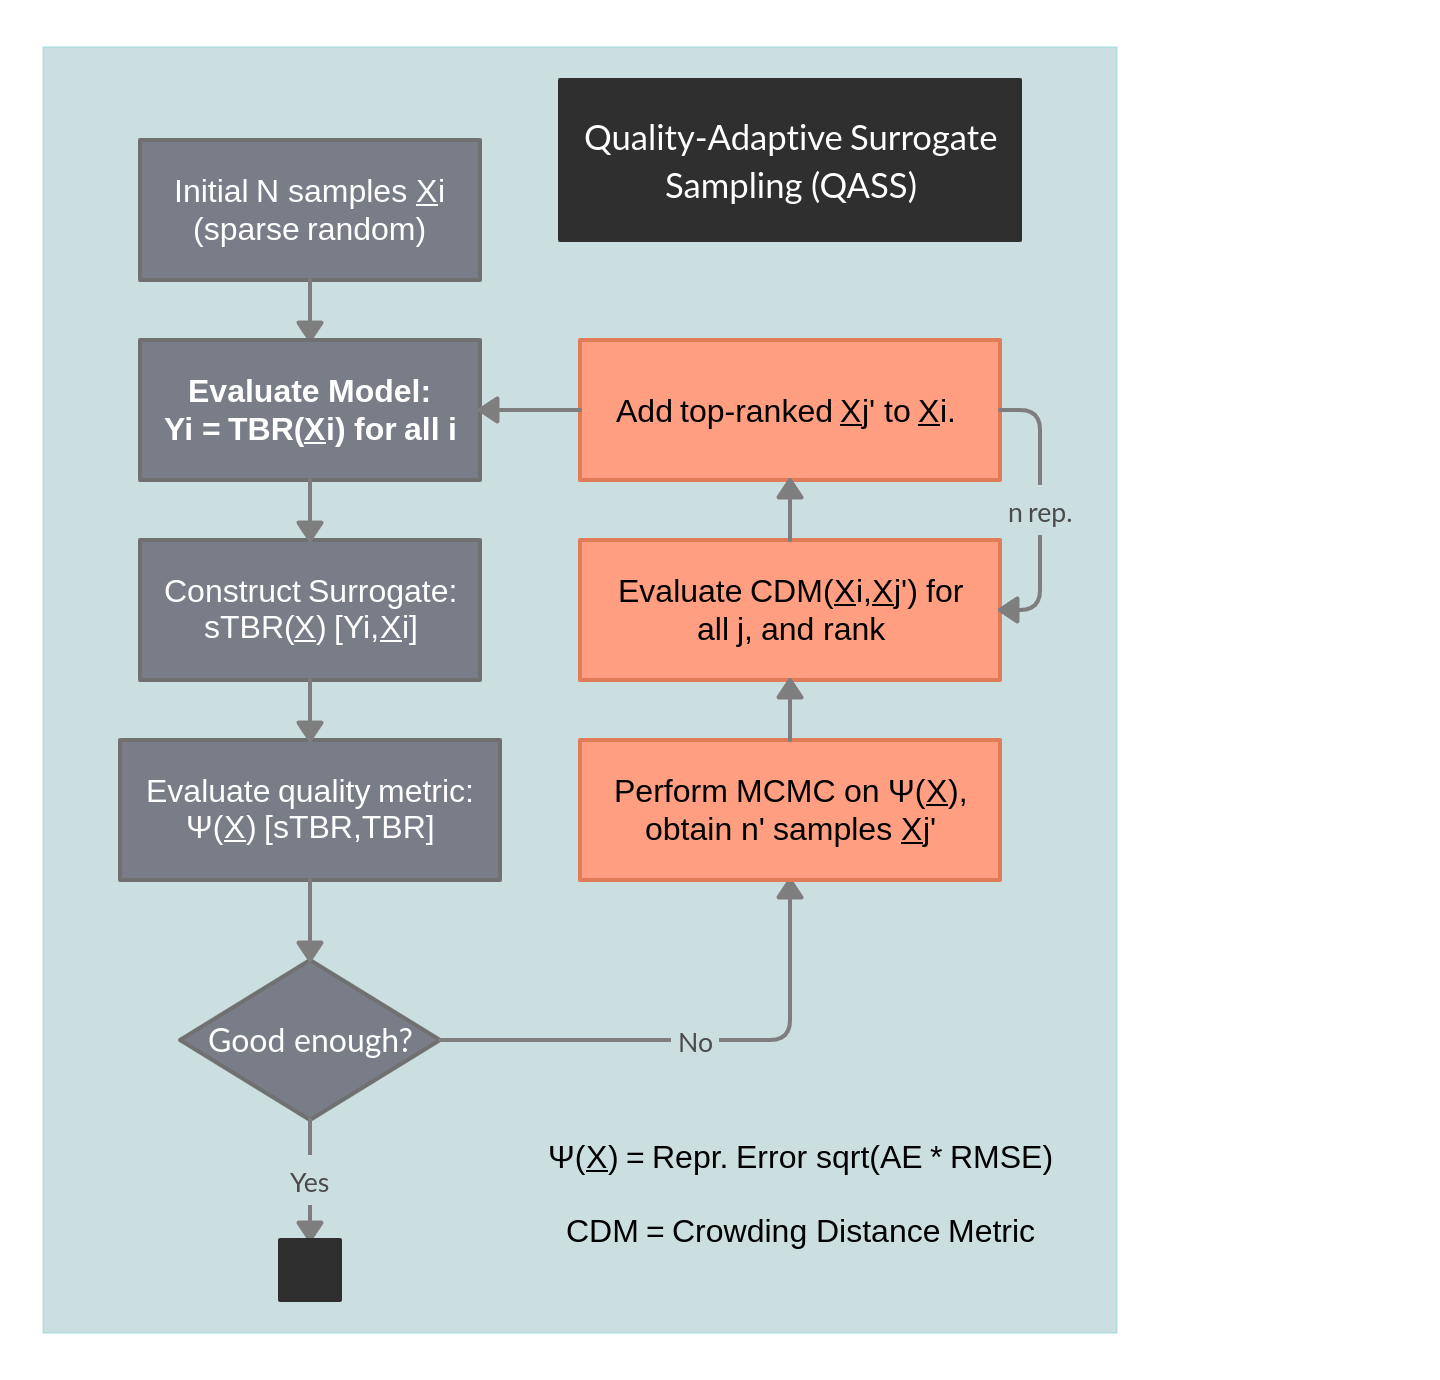
\includegraphics[width=1.2\linewidth]{fig4_qassplan.png}
	\caption{\label{fig:qassplan}Schematic of QASS algorithm}
\end{figure}

Adaptive sampling techniques appear frequently in the literature and have been specialised for surrogate modelling, where precision is implicitly limited by the quantity of training samples which are available from the expensive model. Garud's~\cite{Garud2016} ``Smart Sampling Algorithm'' achieved notable success by incorporating surrogate quality and
crowding distance scoring to identify optimal new samples, but was only tested
on a single-parameter domain. We theorised that a nondeterministic sample
generation approach, built around Markov Chain Monte Carlo methods (MCMC), would
fare better for high-dimensional models by more thoroughly exploring all local
optima in the feature space. MCMC produces each sample points according to a shared proposal
distribution from the prior point. These sample points will converge to a desired posterior
distribution, so long as the acceptance probability meets certain statistical criteria (see~\cite{Zhou2018} for a review).

Many researchers have embedded surrogate methods into MCMC strategies for
parameter optimisation~\cite{Zhang2020,Gong2017}, in particular the ASMO-PODE
algorithm~\cite{Ginting2011} which makes use of MCMC-based adaptive sampling. Our approach draws inspiration from ASMO-PODE, but instead uses MCMC to generate samples
which increase surrogate precision throughout the entire parameter space.

We designed the Quality-Adaptive Surrogate Sampling algorithm (QASS, \fref{fig:qassplan}) to iteratively increment the training/test set with sample
points which maximise surrogate error and minimise a crowding distance metric
(CDM)~\cite{Solonen2012} in feature space. On each iteration following an initial training of the surrogate on $N$ uniformly random samples, the surrogate was trained and absolute error calculated. MCMC was then performed on the error function generated by performing nearest-neighbor interpolation on these test error points. The resultant samples were culled by $50\%$ according to the CDM, and then the $n$ highest-error candidates were selected for reintegration with the training/test set, beginning another training epoch. Validation was also performed during each iteration on independent, uniformly-random sample sets.
